\section{Passo 11 — Gerar o pacote para o VOSviewer}
\label{sec:passo11}

\subsection*{Objetivo}
Exportar o corpus da base final em formato compatível com o VOSviewer e importar de volta o mapa e a
rede para guardar o resultado junto do estudo.

\begin{figure}[H]
\centering
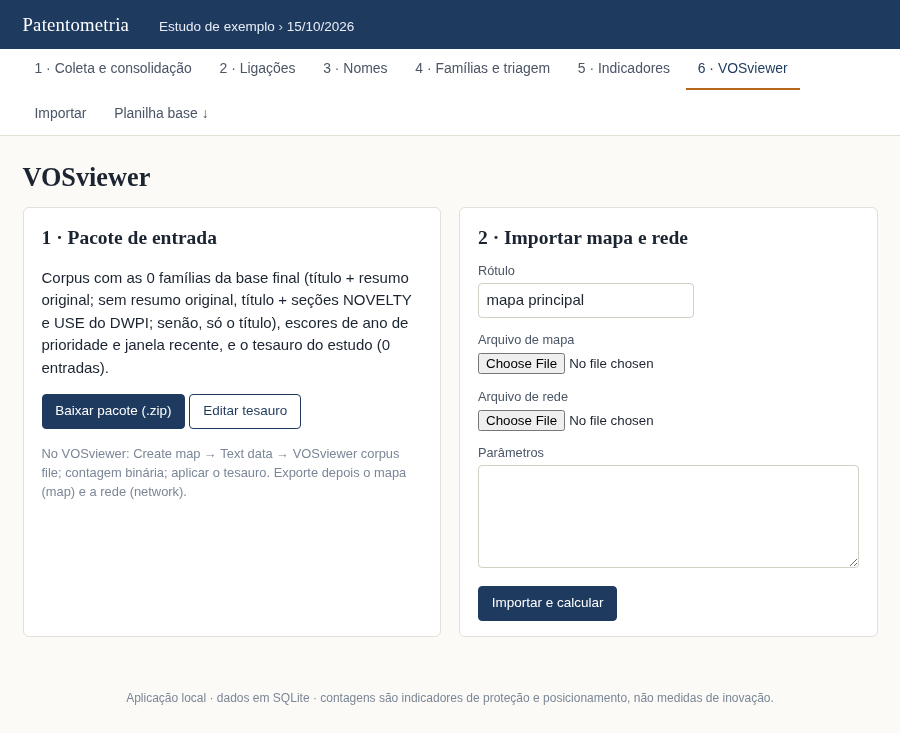
\includegraphics[width=0.9\linewidth]{img/13_vosviewer.png}
\caption{Tela do VOSviewer: geração do pacote de entrada e importação do mapa e da rede já calculados
no programa externo.}
\label{fig:vos}
\end{figure}

\subsection*{O que fazer}
\begin{enumerate}
\item Abra \textbf{VOSviewer} e clique em \textbf{Baixar pacote (.zip)}.
\item No VOSviewer, crie o mapa a partir do arquivo de corpus (Create map $\rightarrow$ Text data).
\item Exporte o mapa e a rede e importe os dois arquivos na aplicação.
\item Descreva os parâmetros usados no campo de observações.
\end{enumerate}

\subsection*{Como interpretar}
O pacote contém título e resumo de cada família da base final, os anos de prioridade e o tesauro do
estudo. Isso significa que o mapa reflete \emph{apenas} o que passou pela triagem --- se a base final
estiver vazia, o corpus sai vazio (é o que acontece na demonstração antes da triagem).

No VOSviewer, a escolha do tipo de análise muda a pergunta: coocorrência de termos descreve o discurso
do corpus; coautoria descreve redes de inventores; citação descreve proximidade entre documentos. O
número mínimo de ocorrências e o tamanho do cluster precisam ser informados no guia do estudo, porque
mudam o desenho.

\begin{nota}[Mapa é exploratório]
Cluster não é categoria analítica validada. Use o mapa para levantar hipóteses e volte aos documentos
para confirmar; não cite o cluster como se fosse um achado.
\end{nota}

\begin{alerta}[Erro comum]
Rodar o VOSviewer na base unificada e apresentar o mapa como se fosse a base final. Os dois conjuntos
respondem a perguntas diferentes.
\end{alerta}

\subsection*{Checkpoint}
\marcador\; O pacote foi gerado, o mapa e a rede estão anexados ao estudo e os parâmetros usados estão
registrados.
